\documentclass[conference]{IEEEtran}
\IEEEoverridecommandlockouts
% \usepackage[utf8]{inputenc}
% \usepackage[brazil]{babel}
% \usepackage[T1]{fontenc}
% \usepackage{lmodern}
\usepackage{hyperref}
\usepackage{graphicx}
\usepackage{amsmath}
\usepackage{amssymb}
% \usepackage{geometry}
\usepackage{listings}
\usepackage{xcolor}
% \usepackage{booktabs}
\usepackage{float}

\usepackage{cite}
\usepackage{amsmath,amssymb,amsfonts}
\usepackage{algorithmic}
\usepackage{graphicx}
\usepackage{textcomp}
\usepackage{xcolor}
\lstdefinestyle{pythonstyle}{
    language=Python,
    basicstyle=\ttfamily\small,
    keywordstyle=\color{blue}\bfseries,
    stringstyle=\color{teal},
    commentstyle=\color{gray}\itshape,
    showstringspaces=false,
    numbers=left,
    numberstyle=\tiny\color{gray},
    stepnumber=1,
    numbersep=8pt,
    frame=single,
    rulecolor=\color{black!30},
    breaklines=true,
    breakatwhitespace=true,
    tabsize=4,
    captionpos=b
}
\geometry{margin=2.5cm}

\title{Atividade 1 Aprendizado Supervisionado \\ \large Relatório de Atividade}
\author{Julio Vinicius Amaral Oliveira \\ Matrícula: 230537 \\ Disciplina: MO432 \\ Professor: Marcos M. Raimundo}
\date{\today}

\begin{document}
\maketitle
\thispagestyle{empty}

\newpage
\tableofcontents
\thispagestyle{empty}

\newpage
\pagenumbering{arabic}

%----------------------------------------
\section{Introdução}
\label{sec:introducao}
\begin{itemize}
  \item O objetivo do trabalho é aplicar técnicas básicas de aprendizado supervisionado para detectar fraudes em transações financeiras. O trabalho foi dividido em duas partes: a primeira parte vamos implementar dois modelos de detecção de fraude, enquanto a segunda parte resolveremos algumas questões teóricas relacionadas ao aprendizado supervisionado.
  \item O dataset utilizado é o Credit Card Fraud Detection. Ele possui transações realizadas com cartões de crédito em setembro de 2013. O conjunto de dados tem a maioria de suas features anonimizadas, com exceção de algumas variáveis como: tempo, valor da transação e a variável que indica se a transação é fraude ou não. Uma característica bem importante desse datasete é que ele é muito desbalanceado, com apenas 0.172\% das transações sendo fraudes.
\end{itemize}

%----------------------------------------
\section{Metodologia (Parte Prática)}
\label{sec:metodologia}

\subsection{Análise Exploratório de Dados (EDA) e Pré-processamento}
\label{subsec:eda}
  Como dito anteriormente, o dataset é bastante desbalanceado, o primeiro passo realizado foi verificar a quantidade de fraudes e não fraudes utilizando o método \texttt{value\_counts()} do pandas. Obtendo o seguinte resultado:
  \begin{figure}[H]
    \centering
    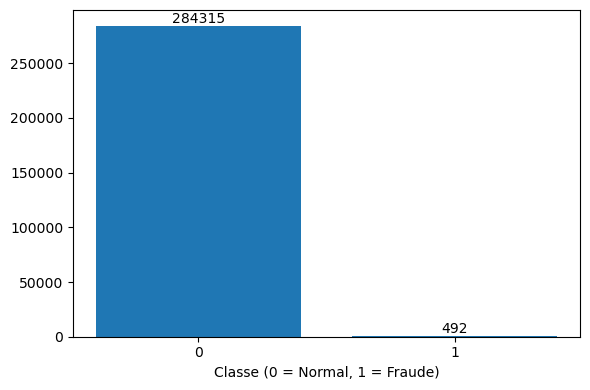
\includegraphics[width=0.8\textwidth]{../output/proporcao_dados.png}
    \caption{Proporção de fraudes e não fraudes no dataset}
    \label{fig:proporcao_dados}
  \end{figure}
  Após isso, procuramos entender como as features se relacionavam com a coluna de Class, que era nossa coluna alvo. Então usamos o método \texttt{corr()} do pandas, buscando a correlação entre Class e o restante das features. obtendo o seguinte resultado para as features com maior correlação absoluta:
  \begin{table}[H]
    \centering
    \begin{tabular}{lr}
        \toprule
        \textbf{Feature} & \textbf{Correlação com Class} \\
        \midrule
        V17    & -0.326481 \\
        V14    & -0.302544 \\
        V12    & -0.260593 \\
        V10    & -0.216883 \\
        V16    & -0.196539 \\
        V3     & -0.192961 \\
        V7     & -0.187257 \\
        \bottomrule
    \end{tabular}
    \caption{Correlação das features com Class}
    \label{tab:correlacao_features}
\end{table}
\subsection{Abordagem 1: Modelagem da Classe Normal (Detecção de Anomalia)}
\label{subsec:abordagem1}
  Para a primeira abordagem utilizamos o modelo de detecção de anomalias. Primeiramente, separamos apenas as 3 features mais relevantes para o modelo, esse número foi escolhido com base na performance do modelo. Foi percebido que ao diminuir cada vez mais o número de features tanto a medida de AUC-PR quanto a matriz de confusão resultavam em valores melhores. Após isso, separamos 2000 transações normais, e com o StandartScaler aplicamos uma normalização para esses dados. Depois aplicamos a normalização para o conjunto inteiro de dados (Com exceção da coluna Class). Após isso, tentamos encontrar o melhor valor de bandwith usando o método \texttt{GridSearchCV} do sklearn. O melhor valor encontrado foi 0.479, e com isso aplicamos um KDE e calculamos o score de anomalias.
\begin{table}[H]
    \centering
  \begin{minipage}{0.48\textwidth}
      \centering
      \begin{tabular}{lrr}
          \toprule
          & \textbf{anomaly\_score} & \textbf{true\_class} \\
          \midrule
          count & 284315.000000 & 284315.0 \\
          mean & 3.818309 & 0.0 \\
          std & 4.005647 & 0.0 \\
          min & 2.346846 & 0.0 \\
          25\% & 2.822756 & 0.0 \\
          50\% & 3.311860 & 0.0 \\
          75\% & 4.210312 & 0.0 \\
          max & 557.518645 & 0.0 \\
          \bottomrule
      \end{tabular}
      \caption{Transações normais}
      \label{tab:score_anomalia_normal}
  \end{minipage}\hfill
  \begin{minipage}{0.48\textwidth}
      \centering
      \begin{tabular}{lrr}
          \toprule
          & \textbf{anomaly\_score} & \textbf{true\_class} \\
          \midrule
          count & 492.000000 & 492.0 \\
          mean & 162.766740 & 1.0 \\
          std & 250.679879 & 0.0 \\
          min & 2.780611 & 1.0 \\
          25\% & 26.711496 & 1.0 \\
          50\% & 68.714390 & 1.0 \\
          75\% & 156.108730 & 1.0 \\
          max & 1377.747682 & 1.0 \\
          \bottomrule
      \end{tabular}
      \caption{Transações fraudulentas}
      \label{tab:score_anomalia_fraude}
  \end{minipage}
\end{table}
Apos isso, tentamos encontrar o melhor limiar para separar as transações, utilizamos o método precision\_recall\_curve do sklearn, e encontramos o melhor limiar para maximizar f1 sendo 34.9 Com isso, conseguimos os seguintes resultados após plotar a matriz de confusão:
\begin{figure}[H]
    \centering
    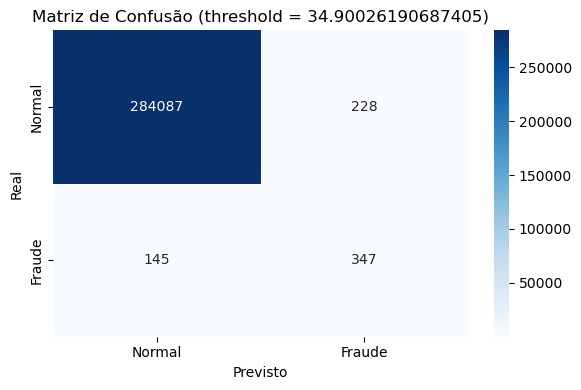
\includegraphics[width=0.8\textwidth]{../output/matriz de confusao maximo f1.png}
    \caption{Matriz de confusão}
    \label{fig:matriz_confusao}
\end{figure}
Segundo o próprio repositório do Kaggle, a matriz de confusão não é o melhor indicador de desempenho quando temos classes desbalanceadas e nesses casos é recomendado o uso da área abaixo da curva de precision-recall. Cujo resultado foi de 0.623
\subsection{Abordagem 2: Classificação Supervisionada}
\label{subsec:abordagem2}
  Nessa segunda abordagem utilizamos um modelo de regressão logística, utilizamos o método train\_test\_split do sklearn para separar 80\% dos dados para treino e 20\% para teste, isso foi realizado nos dados já normalizado com a ajuda do StandartScaler. Após isso, aplicamos o modelo de regressão logística e aplicamos o modelo nos dados de testes, obtendo a seguinte AUC-PR: 0.742, que foi um valor muito maior do que o obtido na primeira abordagem. Para ilustrar também o resultado, plotamos a matriz de confusão:
  \begin{table}[H]
      \centering
      \begin{tabular}{lcccccc}
          \toprule
          & \textbf{Classe 0} & \textbf{Classe 1} & \textbf{Acurácia} & \textbf{Média Macro} & \textbf{Média Ponderada} \\
          \midrule
          Precision   & 0.999 & 0.829 & 0.999 & 0.914 & 0.999 \\
          Recall     & 1.0 & 0.643 & 0.999 & 0.821 & 0.999 \\
          F1-score               & 1.0 & 0.724 & 0.999 & 0.862 & 0.999 \\
          Support      & 56864    & 98       & 0.999 & 56962    & 56962    \\
          \bottomrule
      \end{tabular}
      \caption{Métricas de avaliação do modelo para as classes 0 (normal) e 1 (fraude)}
      \label{tab:metricas_classificacao}
  \end{table}
  \begin{figure}[H]
    \centering
    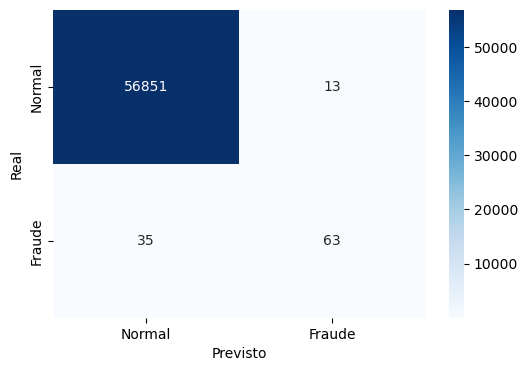
\includegraphics[width=0.8\textwidth]{../output/matriz de confusao sem threshold regressao logistica.png}
    \caption{Matriz de confusão regressão logística}
    \label{fig:matriz_confusao_regressao_logistica}
  \end{figure}
  Para melhorar ainda mais o resultado, resolvemos encontrar um threshold utilizando o método \texttt{precision\_recall\_curve} do sklearn, e ao fazer isso encontramos um valor melhor de recall, entretanto o valor da precision diminuiu um pouco. Mas dado o contexto que o modelo deveria ser usado, ter um recall alto é melhor pois evita perdas financeiras para a empresa que utiliza o modelo, o valores obtidos foram
  \begin{table}[H]
    \centering
    \begin{tabular}{lccccc}
        \toprule
                           & \textbf{Classe 0} & \textbf{Classe 1} & \textbf{Acurácia} & \textbf{Média Macro} & \textbf{Média Ponderada} \\
        \midrule
        Precision  & 0.999  & 0.692  & 0.999  & 0.846  & 0.999   \\
        Recall     & 0.999  & 0.827  & 0.999  & 0.913  & 0.999   \\
        F1-score   & 1.000  & 0.753  & 0.999  & 0.877  & 0.999   \\
        Support    & 56864  & 98     & 56962  & 56962  & 56962   \\
        \bottomrule
    \end{tabular}
    \caption{Métricas de avaliação do modelo (valores aproximados para 3 casas decimais)}
    \label{tab:matriz_confusao_regressao_logistica_com_threshold}
\end{table}
  \begin{figure}[H]
    \centering
    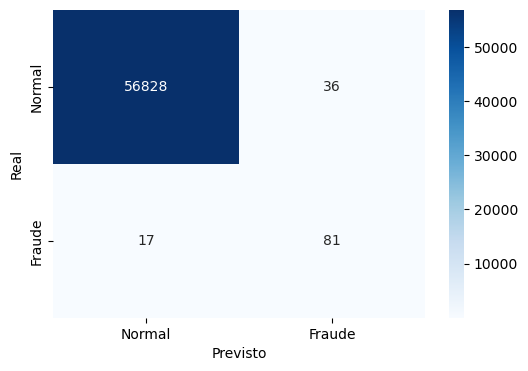
\includegraphics[width=0.8\textwidth]{../output/matriz de confusao com threshold regressao logistica.png}
    \caption{Matriz de confusão regressão logística}
    \label{fig:matriz_confusao_regressao_logistica_com_threshold}
  \end{figure}
\subsection{Uso de LGBM}
\label{subsec:validacao}
Ao utilizar o modelo LGBM, obtivemos um resultado muito superior aos anteriores. Calculamos os scores utilizando o \texttt{predict\_proba} e ajustamos o threshold para maximizar o F1-score. Os thresholds, precision e recall foram encontrados utilizando o método \texttt{precision\_recall\_curve} e calculamos o F1 através da fórmula:
\begin{equation}
    F1 = \frac{2 \cdot (precision \cdot recall)}{precision + recall}
\end{equation}
Seguem os resultados de precisão, recall e F1-score:
\begin{table}[H]
    \centering
    \begin{tabular}{lccccc}
        \toprule
    & \textbf{0} & \textbf{1} & \textbf{Accuracy} & \textbf{macro avg} & \textbf{weighted avg} \\
        \midrule
        Precision  & 1.000 & 0.936 & 1.000 & 0.968 & 1.000 \\
        Recall     & 1.000 & 0.829 & 1.000 & 0.915 & 1.000 \\
        F1‐score   & 1.000 & 0.879 & 1.000 & 0.940 & 1.000 \\
        Support    & 71079 & 123   & 1.000 & 71202 & 71202  \\
        \bottomrule
    \end{tabular}
    \caption{Métricas de avaliação do modelo LGBM}
    \label{tab:metricas_lgbm}
\end{table}
  \begin{figure}[H]
    \centering
    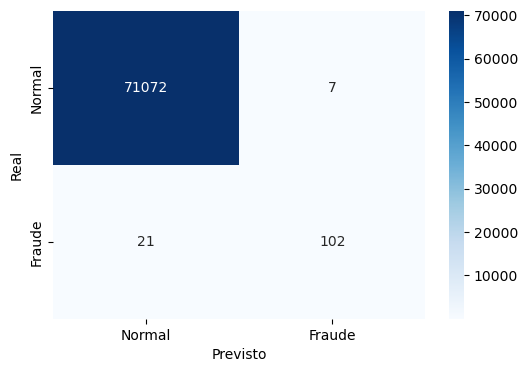
\includegraphics[width=0.8\textwidth]{../output/matriz confusao lgbm.png}
    \label{fig:matriz_confusao_lgbm}
  \end{figure}
Também calculamos a AUC-PR, que foi de 0.8585
A utilização do LGBM trouxe uma distribuição muito heterogênea entre os scores, oque pode ser visto na figura \ref{fig:distribuicao_scores_lgbm}. Enquanto os scores de dados normais se concentram em torno de 0, os scores de dados fraudulentos se concentram em torno de 1, mostrando que o LGBM conseguiu separar bem as classes.
\begin{figure}[H]
    \centering
    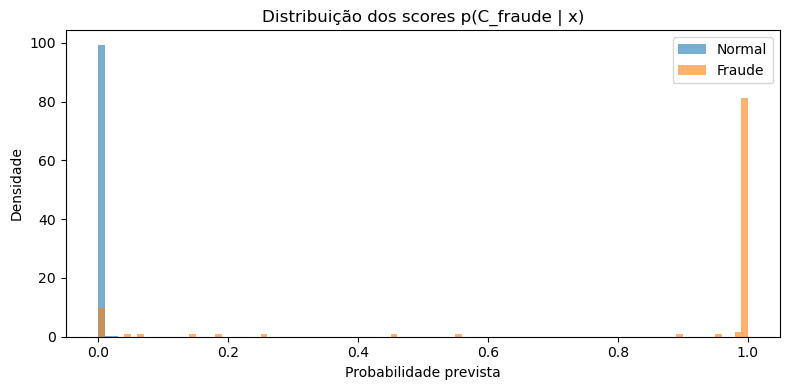
\includegraphics[width=0.8\textwidth]{../output/distribuicao scores lgbm.png}
    \caption{Distribuição dos scores do modelo LGBM}
    \label{fig:distribuicao_scores_lgbm}
\end{figure}
%----------------------------------------

%----------------------------------------
\section{Conclusão}
\label{sec:conclusao}
A primeira abordagem, que utilizou o modelo de detecção de anomalias, obteve um resultado de AUC-PR de 0.623, enquanto a segunda abordagem, que utilizou o modelo de regressão logística, obteve um resultado de AUC-PR de 0.742. Por fim, a terceira abordagem, que utilizou o modelo LGBM, obteve um resultado de AUC-PR de 0.8585. Isso mostra que o modelo LGBM foi o mais eficaz para detectar fraudes no dataset. Deve-se levar em conta também, que na primeira abordagem, o resultado só foi tão alto, devido ao fato de que reduzimos consideravelmente a quantidade de features, pois em testes prévios, ao utilizar todas as features, os resultados eram muito ruins, com AUC-PR próximos de 0.1. A abordagem 2 pareceu melhor, tanto em questão de resultado quanto em questão de performance, já que para realizar a abordagem 1, tivemos que separar um conjunto inferior de dados, utilizar menos features para chegar em um resultado minimamente aceitável. Já na abordagem 2, utilizamos todas as features e mesmo assim chegamos em um resultado muito bom. Quanto a escolha do limiar, utilizamos o método \texttt{precision\_recall\_curve} para encontrar o F1 com maior valor, em um cenário real, talvez o ideal fosse utilizar um limiar que favorecesse ainda mais o recall, dado que estamos lidando com fraudes que podem significar perda financeira para uma empresa, mas ao mesmo tempo é importante considerar que um modelo que tem uma precisão baixa pode causar problemas tanto para clientes que possam ter transações bloqueadas, causando insatisfação quanto para um time que precisará investigar essas transações.

%----------------------------------------
\section{Respostas Teórico-Conceituais (Parte 2)}
\label{sec:teoria}

\subsection{Exercício 1}
\label{subsec:ex1}
\subsection*{(a) Fronteira de Decisão com Covariâncias Diferentes e Priors Iguais}

Sabemos que a probabilidade posterior de uma classe $C_k$ dado um vetor de features $\mathbf{x}$ é dada pelo Teorema de Bayes:
\[
p(C_k | \mathbf{x}) = \frac{p(\mathbf{x} | C_k) p(C_k)}{p(\mathbf{x})}.
\]
A fronteira de decisão é quando $p(C_1 | \mathbf{x}) = p(C_2 | \mathbf{x})$. \\
Segundo o enunciado,  $p(C_1) = p(C_2) = 0.5$. \\

Sabemos que:
\[
\mathcal{N}(\mathbf{x} | \boldsymbol{\mu}_k, \boldsymbol{\Sigma}_k) = \frac{1}{(2\pi)^{D/2} |\boldsymbol{\Sigma}_k|^{1/2}} \exp\left(-\frac{1}{2} (\mathbf{x} - \boldsymbol{\mu}_k)^T \boldsymbol{\Sigma}_k^{-1} (\mathbf{x} - \boldsymbol{\mu}_k)\right) = p(\mathbf{x} | C_k)
\]
Igualando $p(\mathbf{x} | C_1) = p(\mathbf{x} | C_2)$
\[
\frac{p(C_1 | \mathbf{x})p(\mathbf{x})}{p(C_1)} = \frac{p(C_2 | \mathbf{x})p(\mathbf{x})}{p(C_2)} 
\]

Ao simplificar, obtemos:
\[
p(\mathbf{x} | C_1) = p(\mathbf{x} | C_2)
\]
Portanto, igualando a expressão obtida acima e aplicando o logaritmo natural:
\begin{align*}
& -\frac{1}{2} (\mathbf{x} - \boldsymbol{\mu}_1)^T \boldsymbol{\Sigma}_1^{-1} (\mathbf{x} - \boldsymbol{\mu}_1) - \frac{1}{2} \ln |\boldsymbol{\Sigma}_1| \\
&= -\frac{1}{2} (\mathbf{x} - \boldsymbol{\mu}_2)^T \boldsymbol{\Sigma}_2^{-1} (\mathbf{x} - \boldsymbol{\mu}_2) - \frac{1}{2} \ln |\boldsymbol{\Sigma}_2|.
\end{align*}
Dividindo por -1/2 e rearranjando, a equação fica:
\[
(\mathbf{x} - \boldsymbol{\mu}_1)^T \boldsymbol{\Sigma}_1^{-1} (\mathbf{x} - \boldsymbol{\mu}_1) + \ln |\boldsymbol{\Sigma}_1| = (\mathbf{x} - \boldsymbol{\mu}_2)^T \boldsymbol{\Sigma}_2^{-1} (\mathbf{x} - \boldsymbol{\mu}_2) + \ln |\boldsymbol{\Sigma}_2|.
\]
Como $x^T\Sigma^{-1}\mu$ é escalar, $x^T\Sigma^{-1}\mu = (x^T\Sigma^{-1}\mu)^T = \mu ^ T \Sigma ^{-1} x$, expandindo os termos e aplicando essa propriedade, obtemos: 
\[
\mathbf{x}^T \boldsymbol{\Sigma}_1^{-1} \mathbf{x} - 2 \boldsymbol{\mu}_1^T \boldsymbol{\Sigma}_1^{-1} \mathbf{x} + \boldsymbol{\mu}_1^T \boldsymbol{\Sigma}_1^{-1} \boldsymbol{\mu}_1 + \ln |\boldsymbol{\Sigma}_1| = \mathbf{x}^T \boldsymbol{\Sigma}_2^{-1} \mathbf{x} - 2 \boldsymbol{\mu}_2^T \boldsymbol{\Sigma}_2^{-1} \mathbf{x} + \boldsymbol{\mu}_2^T \boldsymbol{\Sigma}_2^{-1} \boldsymbol{\mu}_2 + \ln |\boldsymbol{\Sigma}_2|.
\]
Reorganizando os termos, obtemos:
\[
\mathbf{x}^T (\boldsymbol{\Sigma}_1^{-1} - \boldsymbol{\Sigma}_2^{-1}) \mathbf{x} - 2 (\boldsymbol{\mu}_1^T \boldsymbol{\Sigma}_1^{-1} - \boldsymbol{\mu}_2^T \boldsymbol{\Sigma}_2^{-1}) \mathbf{x} + (\boldsymbol{\mu}_1^T \boldsymbol{\Sigma}_1^{-1} \boldsymbol{\mu}_1 - \boldsymbol{\mu}_2^T \boldsymbol{\Sigma}_2^{-1} \boldsymbol{\mu}_2 + \ln |\boldsymbol{\Sigma}_1| - \ln |\boldsymbol{\Sigma}_2|) = 0.
\]
Essa equação tem um formato de $x^TAx + b^Tx+c = 0$ que é uma superfície quadrática.

\subsection*{(b) Efeito da Alteração do Prior com Covariâncias Compartilhadas}

Como os priors são $p(C_1) = \pi$ e $p(C_2) = 1 - \pi$, tomando a condição para a fronteira de decisão $p(\mathbf{x} | C_1) p(C_1) = p(\mathbf{x} | C_2) p(C_2)$ temos que:
\[
\mathcal{N}(\mathbf{x} | \boldsymbol{\mu}_1, \boldsymbol{\Sigma}) \pi = \mathcal{N}(\mathbf{x} | \boldsymbol{\mu}_2, \boldsymbol{\Sigma}) (1 - \pi).
\]
Aplicando o logaritmo natural nos dois lados:
\begin{align*}
& -\frac{1}{2} (\mathbf{x} - \boldsymbol{\mu}_1)^T \boldsymbol{\Sigma}^{-1} (\mathbf{x} - \boldsymbol{\mu}_1) - \frac{1}{2} \ln |\boldsymbol{\Sigma}| + \ln \pi \\
&= -\frac{1}{2} (\mathbf{x} - \boldsymbol{\mu}_2)^T \boldsymbol{\Sigma}^{-1} (\mathbf{x} - \boldsymbol{\mu}_2) - \frac{1}{2} \ln |\boldsymbol{\Sigma}| + \ln (1 - \pi).
\end{align*}
Expandindo os termos, temos:
\[
-\frac{1}{2} (\mathbf{x}^T \boldsymbol{\Sigma}^{-1} \mathbf{x} - 2 \boldsymbol{\mu}_1^T \boldsymbol{\Sigma}^{-1} \mathbf{x} + \boldsymbol{\mu}_1^T \boldsymbol{\Sigma}^{-1} \boldsymbol{\mu}_1) + \ln \pi = -\frac{1}{2} (\mathbf{x}^T \boldsymbol{\Sigma}^{-1} \mathbf{x} - 2 \boldsymbol{\mu}_2^T \boldsymbol{\Sigma}^{-1} \mathbf{x} + \boldsymbol{\mu}_2^T \boldsymbol{\Sigma}^{-1} \boldsymbol{\mu}_2) + \ln (1 - \pi).
\]
Simplificando e rearranjando, temos:
\[
(\boldsymbol{\mu}_1 - \boldsymbol{\mu}_2)^T \boldsymbol{\Sigma}^{-1} \mathbf{x} - \frac{1}{2} (\boldsymbol{\mu}_1^T \boldsymbol{\Sigma}^{-1} \boldsymbol{\mu}_1 - \boldsymbol{\mu}_2^T \boldsymbol{\Sigma}^{-1} \boldsymbol{\mu}_2) + \ln \left(\frac{\pi}{1 - \pi}\right) = 0.
\]
Essa expressão tem o formato de uma equação:
\begin{align*}
& \omega ^T x + \omega_0 = 0 \\
& \omega_0 = -\frac{1}{2} (\boldsymbol{\mu}_1^T \boldsymbol{\Sigma}^{-1} \boldsymbol{\mu}_1 - \boldsymbol{\mu}_2^T \boldsymbol{\Sigma}^{-1} \boldsymbol{\mu}_2) + \ln \left(\frac{\pi}{1 - \pi}\right)\\
& \omega = \boldsymbol{\Sigma}^{-1} (\boldsymbol{\mu}_1 - \boldsymbol{\mu}_2).
\end{align*}
$\ln \left(\frac{\pi}{1 - \pi}\right)$ é um deslocamento escalar na equação linear. Alterar o prior $\pi$ resulta no deslocamento paralelo da fronteira de decisão.
\begin{itemize}
    \item Se $\pi > 0.5$ ($p(C_1) > p(C_2)$), implica que $\ln \left(\frac{\pi}{1 - \pi}\right) > 0$. Para satisfazer a equação, $(\boldsymbol{\mu}_1 - \boldsymbol{\mu}_2)^T \boldsymbol{\Sigma}^{-1} \mathbf{x}$ precisa ser menor, fazendo com que a fronteira se expanda para a região de $C_1$.
    \item Se $\pi < 0.5$ (ou seja, $p(C_1) < p(C_2)$), então $\ln \left(\frac{\pi}{1 - \pi}\right) < 0$, e a fronteira se desloca na direção oposta, expandindo a região de $C_2$.
    \item Se $\pi = 0.5$, o termo logarítmico é zero, e a fronteira não se desloca para nenhum dos lados, sendo definida pelas médias e covariância.
\end{itemize}

\subsection*{(c) Uso da Distância de Mahalanobis para Classificação:}
A distância de Mahalanobis pode ser usada para classificação comparando a distância de um ponto \(\mathbf{x}\) para os centros das classes (\(\boldsymbol{\mu}_1\) e \(\boldsymbol{\mu}_2\)), ponderadas pelas suas respectivas matrizes de covariância. A regra de classificação seria classificar \(\mathbf{x}\) como pertencente à classe \(C_1\) para a qual a distância de Mahalanobis quadrática \(\Delta_1^2\) é mínima. Ou seja:
\begin{itemize}
    \item Se \(\Delta_1^2 \leqslant \Delta_2^2\), classificar \(\mathbf{x}\) como \(C_1\) (Normal).
    \item Se \(\Delta_1^2 > \Delta_2^2\), classificar \(\mathbf{x}\) como \(C_2\) (Fraude).
\end{itemize}

Premissas Implícitas:
\begin{itemize}
    \item As classes devem seguir uma distribuição Gaussiana multivariada. 
    \item Os parâmetros $\boldsymbol{\mu}_1, \boldsymbol{\Sigma}_1, \boldsymbol{\mu}_2, \boldsymbol{\Sigma}_2$ são conhecidos ou foram bem estimados.
    \item Priors iguais para as classes \(p(C_1) = p(C_2)\).
\end{itemize}

\subsection{Exercício 2: Verossimilhança, entropia cruzada e regressão logística}
\label{subsec:ex2}
\section*{(a) Mostrar que maximizar a função de verossimilhança é equivalente a minimizar a entropia cruzada.}
Para um modelo de regressão logística com alvos binários:
\[
p(\mathbf{t} | \mathbf{w}) = \prod_{n=1}^{N} y_n^{t_n} (1 - y_n)^{1 - t_n}
\]
Sabendo que maximizar a função é o mesmo que maximizar o logaritmo natural, podemos aplicar o logaritmo natural para que a função se pareça mais com o nosso objetivo:
\[
\ln p(\mathbf{t} | \mathbf{w}) = \sum_{n=1}^{N} \ln \left( y_n^{t_n} (1 - y_n)^{1 - t_n} \right).
\]
Usando as propriedades do logaritmo:
\[
\ln p(\mathbf{t} | \mathbf{w}) = \sum_{n=1}^{N} \left[ t_n \ln y_n + (1 - t_n) \ln(1 - y_n) \right].
\]
A função de erro de entropia cruzada é definida por:
\[
E(\mathbf{w}) = -\sum_{n=1}^{N} \left[ t_n \ln y_n + (1 - t_n) \ln(1 - y_n) \right].
\]
Comparando as duas equações, vemos que $E(\mathbf{w}) = -\ln p(\mathbf{t} | \mathbf{w})$. Portanto, maximizar a verossimilhança é equivalente a minimizar a entropia cruzada.

\section*{(b) Derivando $\nabla E(\mathbf{w})$}
Lembrando que $y_n = \sigma(\mathbf{a}_n)$, com $\mathbf{a}_n = \mathbf{w}^T \boldsymbol{\phi}_n$, e que
\[
\frac{d\sigma(a)}{da} = \sigma(a)(1 - \sigma(a)),
\]
a função de erro é:
\[
E(\mathbf{w}) = -\sum_{n=1}^{N} \left[ t_n \ln \sigma(\mathbf{w}^T \boldsymbol{\phi}_n) + (1 - t_n) \ln(1 - \sigma(\mathbf{w}^T \boldsymbol{\phi}_n)) \right].
\]
O gradiente de $E(\mathbf{w})$ é:
\begin{align*}
\nabla E(\mathbf{w}) &= -\sum_{n=1}^{N} \left[ t_n \frac{1}{y_n} y_n (1 - y_n) \boldsymbol{\phi}_n + (1 - t_n) \frac{1}{1 - y_n} (-y_n (1 - y_n)) \boldsymbol{\phi}_n \right] \\
&= -\sum_{n=1}^{N} \left[ t_n (1 - y_n) - (1 - t_n) y_n \right] \boldsymbol{\phi}_n \\
&= \sum_{n=1}^{N} (y_n - t_n) \boldsymbol{\phi}_n.
\end{align*}

\section*{(c) Explicação do problema de overfitting}
O overfitting ocorre quando os dados são linearmente separáveis. Nesse caso, existe um $\mathbf{w}$ tal que $\mathbf{w}^T \boldsymbol{\phi}_n$ separa perfeitamente as classes, fazendo com que $\|\mathbf{w}\| \to \infty$.

Para evitar isso, usa-se regularização $L_2$:
\[
E_{\text{regularizado}}(\mathbf{w}) = -\sum_{n=1}^{N} \left[ t_n \ln y_n + (1 - t_n) \ln(1 - y_n) \right] + \frac{\lambda}{2} \|\mathbf{w}\|^2,
\]
O termo $\frac{\lambda}{2} \|\mathbf{w}\|^2$ penaliza pesos grandes, fazendo com que o modelo faça um overfitting.

\subsection{Exercício 3: Decomposição viés-variância}
\label{subsec:ex3}
\subsection*{(a) Explicação $(bias) ^ 2$ , variance e noise}
\paragraph{$Bias ^ 2$}
O viés quadrático mede o erro sistemático do modelo, ou seja, o quanto em média o modelo se difere do valor real. Um modelo com um viés alto não consegue entender a complexidade dos dados, levando a um underfitting.
\paragraph{Variance}
A variância mede o quanto as nossas predições pra um dado ponto variam usando diferentes conjuntos de treino. Um modelo que tem alta variância é muito sensível às variações nos dados de treino, fazendo com que o modelo não consiga performar bem em dados que ele não conhece, levando a um overfitting.
\paragraph{Noise}
O ruído é a parte do erro que não é possível de ser reduzida, pois ele é uma característica inerente aos dados.
\subsection*{(b) Explicação $(bias) ^ 2$ , variance e noise}
\subsection{Exercício 4: Avaliação em dados desbalanceados}

\subsection*{(a) Acurácia padrão em datasets desbalanceados}
Em dados desbalanceados, a acurácia padrão pode dar uma falsa sensação que um modelo está muito bom. Já que um classificador simples que sempre classifica as transações como a classe majoritária pode ter uma alta acurácia pois ele irá classificar corretamente na grande maioria das vezes. Isso acontence porque a acurácia é definida como:
\[
\text{Acurácia} \;=\;
\frac{\text{TP} + \text{TN}}{\text{TP} + \text{TN} + \text{FP} + \text{FN}}
\]
Em datasets desbalanceados, a classe majoritária tem um peso muito grande sobre essa métrica. Sendo assim, o classificador não cumpriria seu objetivo que é identificar fraudes, porém  ainda sim teria uma acurácia alta.

\subsection*{(b) Precisão, Recall e F1-Score}

\begin{description}
  \item[Precision] 
    Parcela das transações classificadas como fraude e que de fato são fraude:
    \[
      \text{Precision} \;=\;
      \frac{\text{TP}}{\text{TP} + \text{FP}}
    \]
    Em que:
    \begin{itemize}
      \item TP: quantidade de fraudes classificadas corretamente.
      \item FP: quantidade de transações normais classificadas como fraude.
    \end{itemize}

  \item[Recall]
    Parcela de todas as transações que de fato eram fraudes que foram classificadas corretamente:
    \[
      \text{Recall} \;=\;
      \frac{\text{TP}}{\text{TP} + \text{FN}}
    \]
    Em que:
    \begin{itemize}
      \item FN: quantidade de fraudes que foram classificadas como transações normais.
    \end{itemize}

  \item[F1-Score (\(F_1\))]
    Média harmônica entre precisão e recall:
    \[
      F_1 \;=\;
      2 \,\frac{\text{Precision}\,\times\,\text{Recall}}
             {\text{Precision} + \text{Recall}}
    \]
\end{description}

\paragraph{Quando priorizar Recall sobre Precisão}
\begin{itemize}
  \item Em situações em que perder uma fraude gera prejuízo financeiro para a empresa que utiliza o classificador ou em cenários em que uma classificação errada pode gerar muito prejuízo para o utilizador, como em resultado de doenças.
\end{itemize}

\paragraph{Quando priorizar Precisão sobre Recall}
\begin{itemize}
  \item Quando o custo de falsos positivos é alto, seja por implicar em esforço manual, gerar insatisfação ou diminuir a confiança do cliente nos serviços oferecidos pela empresa que se utiliza do classificador. Além disso, para que a precisão tenha mais relevância que o recall, é necessário que o impacto de um falso negativo não seja tão alto para o negócio. Por exemplo, em um sistema de identificação de câncer, um falso negativo poderia levar a um diagnóstico mais tardio da doença.
\end{itemize}

\subsection*{(c) Curva Precisão–Recall e AUC–PR}

O procedimento para calcular a curva PR seria:

\begin{enumerate}
  \item Ordenar todos os exemplos em ordem decrescente dos seus scores \(s_n\).
  \item Para cada limiar \(\tau\):
    \begin{itemize}
      \item Classificar \(x_n\) como fraude se \(s_n \ge \tau\), caso contrário, classificar como normal.
      \item Calcular
    \[
        \text{Precision}(\tau)
        = \frac{\#\{n : s_n \ge \tau,\; t_n=1\}}
               {\#\{n : s_n \ge \tau\}},
        \quad
        \text{Recall}(\tau)
        = \frac{\#\{n : s_n \ge \tau,\; t_n=1\}}
               {\#\{n : t_n=1\}}.
      \]
    \end{itemize}
  \item Plotar cada ponto do par ($Recall(\tau)$ , $Precision(\tau)$) e formar a curva.
\end{enumerate}

A área Sob a Curva PR é dada por
\[
  \mathrm{AUC\text{-}PR}
  = \int_{0}^{1} \! \text{Precision}(r)\,\mathrm{d}r,
\]
em que \(\text{Precision}(r)\) é a precisão correspondente ao recall \(r\).

\paragraph{Por que AUC–PR é preferível à ROC em cenários muito desbalanceados}
  A curva ROC avalia a taxa de verdadeiros positivos e falsos positivos, em casos desbalanceados a taxa de falsos positivo
  \[
  FPR = \frac{FP}{FP + TN}
  \]
  Permanece baixa pois a quantidade de verdadeiro negativos é muito alta, então essa métrica mascara um modelo ruim. Enquanto a AUC-PR avalia diretamente os dados de fraude, ou seja, não temos um denominador muito alto que mascara o valor da métrica. 


\section{Referências}
\label{sec:referencias}
% Exemplo de uso de BibTeX:
% \bibliographystyle{ieeetr}
% \bibliography{referencias}
\appendix
\section{Correlação das Features com Class}
\label{apendice:correlacao}

\begin{table}[H]
    \centering
    \begin{tabular}{lr}
        \toprule
        \textbf{Feature} & \textbf{Correlação com Class} \\
        \midrule
        V17    & -0.326481 \\
        V14    & -0.302544 \\
        V12    & -0.260593 \\
        V10    & -0.216883 \\
        V16    & -0.196539 \\
        V3     & -0.192961 \\
        V7     & -0.187257 \\
        V11    &  0.154876 \\
        V4     &  0.133447 \\
        V18    & -0.111485 \\
        V1     & -0.101347 \\
        V9     & -0.097733 \\
        V5     & -0.094974 \\
        V2     &  0.091289 \\
        V6     & -0.043643 \\
        V21    &  0.040413 \\
        V19    &  0.034783 \\
        V20    &  0.020090 \\
        V8     &  0.019875 \\
        V27    &  0.017580 \\
        Time   & -0.012323 \\
        V28    &  0.009536 \\
        V24    & -0.007221 \\
        Amount &  0.005632 \\
        V13    & -0.004570 \\
        V26    &  0.004455 \\
        V15    & -0.004223 \\
        V25    &  0.003308 \\
        V23    & -0.002685 \\
        V22    &  0.000805 \\
        \bottomrule
    \end{tabular}
    \caption{Correlação das features com a variável Class}
    \label{tab:correlacao_features_completa}
\end{table}

\end{document}
